%This is the first chapter of the dissertation

%The following command starts your chapter. If you want different titles used in your ToC and at the top of the page throughout the chapter, you can specify those values here. Since Columbia doesn't want extra information in the headers and footers, the "Top of Page Title" value won't actually appear.

\chapter[Supersymmetry][Top of Page Title]{Supersymmetry}\label{ch:susy}

This chapter will introduce supersymmetry (SUSY) ~\cite{Miyazawa:1966mfa, Gervais:1971xj, Gervais:1971ji, Golfand:1971iw, Neveu:1971rx, Neveu:1971iv, Volkov:1973ix,  Wess:1973kz, Salam:1974ig, Ferrara:1974ac, Wess:1974tw, susyPrimer,Lykken:1996xt, archilSUSYLectures}.
We will begin by introducing the concept of a \textit{superspace}, and discuss some general ingredients of supersymmetric theories.
This will include a discussion of how the problems with the Standard Model described in \Cref{ch:sm} are naturally fixed by these theories.

The next step is to discuss the particle content of the \textit{Minimally Supersymmetric Standard Model} (MSSM).
As its name implies, this theory contains the minimal additional particle content to make Standard Model supersymmetric.
We then discuss the important phenomenological consequences of this theory, especially as it would be observed in experiments at the LHC.

\section{Supersymmetric theories : from space to superspace}

\subsection{Coleman-Mandula ``no-go'' theorem}

We begin the theoretical motivation for supersymmetry by citing the ``no-go'' theorem of Coleman and Mandula ~\cite{Coleman:1967ad}.
This theorem forbids \textit{spin-charge unification}.
It states that all quantum field theories which contain nontrivial interactions must be a direct product of the \Poincare~ group of Lorentz symmetries, the internal product of gauge symmetries, and the discrete symmetries of parity, charge conjugation, and time reversal.
The assumptions which go into building the Coleman-Mandula theorem are quite restrictive, but there is solution, which has become known as \textit{supersymmetry} ~\cite{Golfand:1971iw, Haag:1974qh}.
In particular, we must introduce a \textit{spinorial} group generator $Q$.
Alternatively, and equivalently, this can be viewed as the addition of anti-commuting coordinates.
Space plus these new anti-commuting coordinates is then called \textit{superspace} ~\cite{Salam:1974jj}.
We will not investigate this view in detail, but it is also a quite intuitive and beautiful way to construct supersymmetry~\cite{susyPrimer}.

\subsection{Supersymmetry transformations}

A \textit{supersymmetric} transformation $Q$ transforms a bosonic state into a fermionic state, and vice versa :
\begin{align}
Q \ket{\text{Fermion}} &= \ket{\text{Boson}} \\
Q \ket{\text{Boson}} &= \ket{\text{Fermion}}
\end{align}
To ensure this relation holds, $Q$ must be an anticommuting spinor.
Additionally, since spinors are inherently complex, $Q^\dagger$ must also be a generator of the supersymmetry transformation.
Since $Q$ and $Q^\dagger$ are spinor objects (with $s = 1/2$), we can see that supersymmetry must be a spacetime symmetry.
The Haag-Lopuszanski-Sohnius extension ~\cite{Haag:1974qh} of the Coleman-Mandula theorem ~\cite{Coleman:1967ad} is quite restrictive about the forms of such a symmetry.
Here, we simply write the (anti-) commutation relations ~\cite{susyPrimer} :
\begin{align}
{Q_\alpha, Q_{\dot{\alpha}}^\dagger} &= -2 \sigma_{\alpha \dot{\alpha}^\mu} P_\mu \\
{Q_\alpha,Q_{\dot{\beta}}} &= {Q_{\dot{\alpha}}^\dagger, Q_{\dot{\beta}}^\dagger}  = 0 \\
[P^\mu , Q_{\alpha} ] &= [P^\mu, Q_{\dot{\alpha}}^\dagger] = 0
\end{align}

\subsection{Supermultiplets}\label{subsec:supermultiplets}

In a supersymmetric theory, we organize single-particle states into irreducible representations of the supersymmetric algebra which are known as \textit{supermultiplets}.
Each supermultiplet contains a fermion state $\ket{\text{F}}$ and a boson state $\ket{\text{B}}$
These two states are the known as \textit{superpartners}.
These are related by some combination of $Q$ and $Q^\dagger$, up to a spacetime transformation.
$Q$ and $Q^\dagger$ commute with the mass-squared operator $-P^2$ and the operators corresponding to the gauge transformations ~\cite{susyPrimer}: in particular, the gauge interactions of the Standard Model.
In an unbroken supersymmetric theory, this means the states $\ket{\text{F}}$ and $\ket{\text{B}}$ have exactly the same mass, electromagnetic charge, electroweak isospin, and color charges.
One can also prove ~\cite{susyPrimer} that each supermultiplet contains the exact same number of bosonic ($n_B$) and fermion ($n_F$) degrees of freedom.
We now explore the possible types of supermultiples one can find in a renormalizable supersymmetric theory.

Since each supermultiplet must contain a fermion state, the simplest type of supermultiplet contains a single Weyl fermion state ($n_F = 2$) which is paired with $n_B = 2$ scalar bosonic degrees of freedom.
This is most conveniently constructed as single complex scalar field.
We call this construction a \textit{scalar supermultiplet} or \textit{chiral supermultiplet}.
The second name is indicative, as only chiral supermultiplets can contain fermions whose right-handed and left-handed components transform differently under the gauge interactions (as of course happens in the Standard Model).

The second type of supermultiplet we construct is known as a \textit{gauge} supermultiplet.
We take a spin-1 gauge boson (which must be massless due to the gauge symmetry, so $n_B = 2$) and pair this with a single massless Weyl spinor\footnotemark.
\footnotetext{Choosing an $s = 3/2$ massless fermion leads to nonrenormalizable interactions.}
The gauge bosons transform as the adjoint representation of the their respective gauge groups
Their fermionic partners, which are known as gauginos, must also.
In particular, the left-handed and right-handed components of the gaugino fermions have the same gauge transformation properties.

Excluding gravity, this is the entire list of supermultiplets which can participate in renormalizable interactions in what is known as $N=1$ supersymmetry.
This means there is only one copy of the supersymmetry generators $Q$ and $Q^\dagger$.
This is essentially the only ``easy'' phenomenological choice, since it is the only option in four dimensions which allows for the chiral fermions and parity violations to be built into the Standard Model.
We will not look further into $N>1$ supersymmetry in this thesis.

The primary goal, after understanding the possible structures of the multiplets above, is to fit the Standard Model particles into a multiplet, and therefore make predictions about their supersymmetric partners.
We explore this in the next section.

\section{Minimally Supersymmetric Standard Model}

To construct what is known as the MSSM ~\cite{Dimopoulos:1981zb,Dimopoulos:1981yj,Ibanez:1981yh,Marciano:1981un,susyPrimer}, we need a few ingredients and assumptions.
First, we match the Standard Model particles with their corresponding superpartners of the MSSM.
We will also introduce the naming of the superpartners (also known as \textit{sparticles}).
We discuss a very common additional restraint imposed on the MSSM, known as $R$-parity.
We also discuss the concept of soft supersymmetry breaking and how it manifests itself in the MSSM.

\subsection{Chiral supermultiplets}

The first thing we deduce is directly from \Cref{subsec:supermultiplets}.
The bosonic superpartners associated to the quarks and leptons \textit{must} be spin 0, since the quarks and leptons must be arranged in a chiral supermultiplet.
This is essential, since the chiral supermultiplet is the only one which can distinguish between the left-handed and right-handed components of the Standard Model particles.
The superpartners of the quarks and leptons are known as \textit{squarks} and \textit{sleptons}, or \textit{sfermions} in aggregate. (for ``scalar quarks'', ``scalar leptons'', and ``scalar fermion'').
The ``s-'' prefix can also be added to the individual quarks i.e. \textit{selectron}, \textit{sneutrino}, and \textit{stop}.
The notation is to add a $\order$ over the corresponding Standard Model particle i.e. $\supe{e}$, the selectron is the superpartner of the electron.
The two-component Weyl spinors of the Standard Model must each have their own (complex scalar) partner i.e. $e_L, e_R$ have two distinct partners : $\supe{e_L} ,\supe{e_R}$.
As noted above, the gauge interactions of any of the sfermions are identical to those of their Standard Model partners.

Due to the scalar nature of the Higgs, it must obviously lie in a chiral supermultiplet.
To avoid gauge anomalies and ensure the correct Yukawa couplings to the quarks and leptons~\cite{susyPrimer}, we must add additional Higgs bosons to any supersymmetric theory.
In the MSSM, we have two chiral supermultiplets.
The SM (SUSY) parts of the multiplets are denoted $H_u (\supe{H_u})$ and $H_d (\supe{H_d})$.
Writing out $H_u$ and $H_d$ explicitly:
\begin{align}
H_u &= \begin{pmatrix} H_u^+ \\ H_u^0 \end{pmatrix}\\
H_d &= \begin{pmatrix} H_d^0 \\ H_d^- \end{pmatrix}
\end{align}
we see that $H_u$ looks very similar to the SM Higgs with $Y = 1$, and $H_d$ is symmetric with $+ \rightarrow -$ and $ Y = -1$.
%$H_u$ is essentially a copy of the SM Higgs $H_u = \$, while $H_d$ an $SU(2)_L$ doublet and $H_d$  have $Y = \pm 1 respectively.
% \footnotemark.
% \footnotetext{This is also quite nice.  In the Standard Model we arbitrarily make the $Y=1/2$ choice for the scalar Higgs}.
The SM Higgs boson, $h_0$, is a linear superposition of the neutral components of these two doublets.
The SUSY parts of the Higgs multiplets, \supe{H_u} and \supe{H_d}, are each left-handed Weyl spinors.
For generic spin-1/2 sparticles, we add the ``-ino'' suffix.
We then call the partners of the two Higgs collectively the \textit{Higgsinos}.

\subsection{Gauge supermultiplets}

The superpartners of the gauge bosons must all be in gauge supermultiplets since they contain a spin-1 particle.
Collectively, we refer to the superpartners of the gauge bosons as the gauginos.

The first gauge supermultiplet contains the gluon, and its superpartner, which is known as the \textit{gluino}, denoted $\supe{g}$.
The gluon is of course the SM mediator of $SU(3)_C$
The gluino is also a colored particle, subject to $SU(3)_C$.
From the SM before EWSB, we have the four gauge bosons of the electroweak symmetry group $SU(2)_L \otimes U(1)_Y : W^{1,2,3}$ and $B^0$.
The superpartners of these particles are thus the \textit{winos} $\supe{W^{1,2,3}}$ and \textit{bino} $\supe{B^0}$, where each is placed in another gauge supermultiplet with its corresponding SM particle.
After EWSB, without breaking supersymmetry, we would also have the zino $\supe{Z^0}$ and photino $\supe{\gamma}$.

The entire particle content of the MSSM can be seen in \Cref{fig:mssm}.
\begin{figure}
\caption{Particles of the MSSM} \label{fig:mssm}
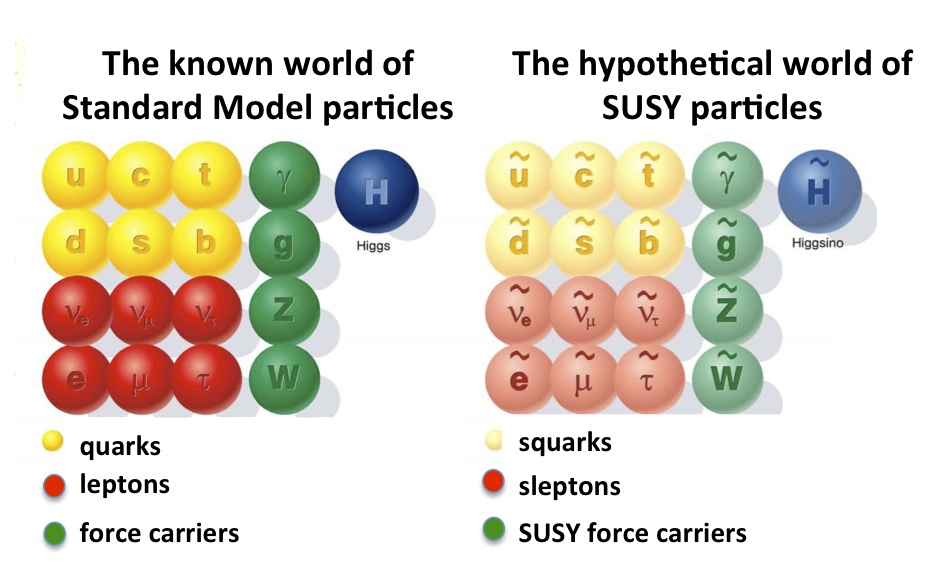
\includegraphics[width=.9\linewidth]{mssm}
\end{figure}

At this point, it's important to take a step back.
Where are these particles?
As stated above, supersymmetric theories require that the masses and all quantum numbers of the SM particle and its corresponding sparticle are the same.
Of course, we have not observed a selectron, squark, or wino.
The answer, as it often is, is that supersymmetry is \textit{broken} by the vacuum state of nature ~\cite{susyPrimer}.

\subsection{$R$-parity}\label{sec:r_parity}

This section is a quick aside to the general story.
$R-parity$ refers to an additional discrete symmetry which is often imposed on supersymmetric models.
For a given particle state, we define
\begin{equation}
R = (-1)^{3(B-L) + 2s}
\end{equation}
where $B,L$ is the baryon (lepton) number and $s$ is the spin.
The imposition of this symmetry forbids certain terms from the MSSM Lagrangian that would violate baryon and/or lepton number.
This is required in order to prevent proton decay, as shown in \Cref{fig:proton_decay}\footnotemark.
\footnotetext{Proton decay can actually be prevented by allowing only one of the four potential R-parity violating terms to survive.}.
\begin{figure}
\caption{This Feynman diagram shows how proton decay is induced in the MSSM, if one does not impose $R$-parity.}\label{fig:proton_decay}
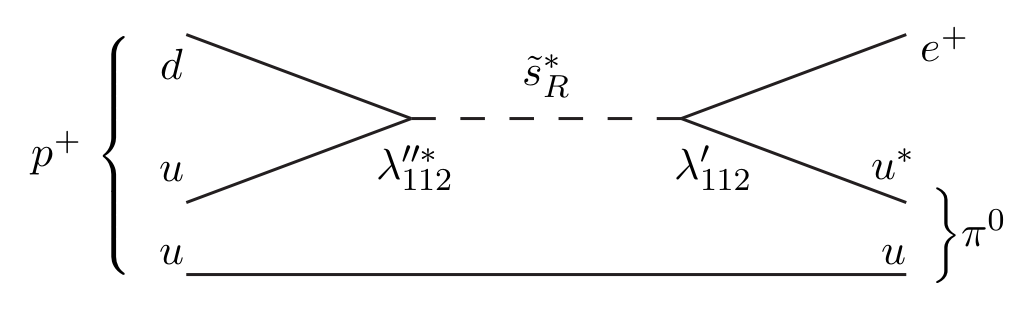
\includegraphics[width=.9\linewidth]{proton_decay}
\end{figure}

In supersymmetric models, this is a $\mathbb{Z}_2$ symmetry, where SM particles have $R=1$ and sparticles have $R=-1$.
We will take $R-parity$ as part of the definition of the MSSM.
We will discuss later the \textit{drastic} consequences of this symmetry on SUSY phenomenology

\subsection{Soft supersymmetry breaking}

The fundamental idea of \textit{soft} supersymmetry breaking~\cite{Girardello:1981wz,,Lykken:1996xt,Chung:2003fi, susyPrimer,archilSUSYLectures} is that we would like to break supersymmetry without reintroducing the quadratic divergences we discussed at the end of Chapter \Cref{ch:sm}.
We write the Lagrangian in a form :
\begin{equation}
\Lagr_{\text{MSSM}} = \Lagr_{\text{SUSY}} + \Lagr_{\text{soft}}
\end{equation}
In this sense, the symmetry breaking is ``soft'', since we have separated out the completely symmetric terms from those soft terms which will not allow the quadratic divergences to the Higgs mass.

The explicitly allowed terms in the soft-breaking Lagrangian are~\cite{archilSUSYLectures}:
\begin{itemize}
\item Mass terms for the scalar components of the chiral supermultiplets
\item Mass terms for the Weyl spinor components of the gauge Supermultiplets
\item Trilinear couplings of scalar components of chiral supermultiplets
\end{itemize}
In particular, using the field content described above for the MSSM, the softly-broken portion of the MSSM Lagrangian can be written
\begin{align}
\Lagr_{\text{soft}} = &-\frac{1}{2}\begin{pmatrix} M_3 \supe{g} \supe{g} + M_2 \supe{W} \supe{W} + M_1 \supe{B} \supe{B} + c.c. \end{pmatrix} \\
                    &-\begin{pmatrix} \supe{u} a_u \supe{Q} H_u - \supe{d} a_d \supe{Q} H_d - \supe{e} a_e \supe{L} H_d + c.c. \end{pmatrix} \\
                    &- \supe{Q}^\dagger m_Q^2 \supe{Q} - \supe{L}^\dagger m_L^2 \supe{L} - \supe{u} m_u^2 \supe{u}^\dagger - \supe{d} m_d^2 \supe{d}^\dagger - \supe{e} m_e^2 \supe{e}^\dagger \\
                    &- m^2_{H_u} H_u^* H_u - m^2_{H_d} H_d^* H_d - (b H_u H_d + cc).
\end{align}
where we have introduced the following notations :
\begin{enumerate}
\item $M_3,M_2,M_1$ are the gluino, wino, and bino masses. \label{list:gaugino_masses}
\item $a_u,a_d,a_e$  are complex $3 \times 3$ matrices in family space. \label{list:yukawa_couplings}
\item $m_Q^2 , m_u^2, m_d^2, m_L^2,m_e^2 $ are hermitian  $3 \times 3$ matrices in family space. \label{list:flavor_changing}
\item $m_{H_u}^2, m_{H_u}^2, b$ are the SUSY-breaking contributions to the Higgs potential. \label{list:higgs}
\end{enumerate}
We have written matrix terms without any sort of additional notational decoration to indicate their matrix nature, and we now show why.
The first term \Cref{list:gaugino_masses} is the set of mass terms for the gluino, wino, and bino.
The second term \Cref{list:yukawa_couplings}, containing $a_u,a_d,a_e$, has strong constraints from experiments ~\cite{Hisano:1995nq,Gabbiani:1996hi}.
We will assume that each $a_i, i = u,d,e$ is proportional to the Yukawa coupling matrix : $a_i = A_{i0} y_i$.
The third term \Cref{list:flavor_changing} can be similarly constrained by experiments ~\cite{ Dimopoulos:1981zb, Gabbiani:1988rb, Hagelin:1992tc, Hagelin:1994id, Choudhury:1994pn, Barbieri:1994pv, deCarlos:1995ah, Casas:1996de,  Gabbiani:1996hi}.
We will assume the elements of the fourth term \Cref{list:higgs} contributing to the Higgs potential as well as all of the \Cref{list:gaugino_masses} terms must be real, which limits the possible CP-violating interactions to those of the Standard Model.
We thus only consider flavor-blind, CP-conserving interactions within the MSSM.

The important mixing for mass and gauge interaction eigenstates in the MSSM occurs within electroweak sector, in a process akin to EWSB in the Standard Model.
The neutral portions of the Higgsinos doublets and the neutral gauginos ($\supe{H^0_u}, \supe{H^0_d} ,\supe{B^0}, \supe{W^0}$) of the gauge interaction basis mix to form what are known as the \textit{neutralinos} of mass basis :
\begin{equation}
M_{\supe{\chi}}=
\begin{pmatrix}
M_1              & 0                & -c_\beta s_W m_Z & s_\beta s_W m_Z  \\
0                & M_2              & c_\beta c_W m_Z  & -s_\beta c_W m_Z \\
-c_\beta s_W m_Z & c_\beta c_W m_Z  & 0                & -\mu             \\
s_\beta s_W m_Z  & -s_\beta c_W m_Z & -\mu             & 0                \\
\end{pmatrix}
\end{equation}
where $s (c)$ are the sine and cosine of angles related to EWSB, which introduced masses to the gauginos and higgsinos.
Diagonalization of this matrix gives the four neutralino mass states, listed without loss of generality in order of increasing mass : $\supe{\chi^0_{1,2,3,4}}$.

The neutralinos, especially the lightest neutralino \lsp, are important ingredients in SUSY phenomenology.

The same process can be done for the electrically charged gauginos with the charged portions of the Higgsino doublets along with the charged winos ($\supe{H^+_u}, \supe{H^+_d}, \supe{W^+}, \supe{W^-}$).
This leads to the \textit{charginos}, again in order of increasing mass : $\supe{\chi_{1,2}^\pm}$.

\section{Phenomenology}

We are finally at the point where we can discuss the phenomenology of the MSSM, in particular as it manifests itself at the energy scales of the LHC.

As noted above in \Cref{sec:r_parity}, the assumption of $R$-parity has important consequences for MSSM phenomenology.
The SM particles have $R=1$, while the sparticles all have $R=-1$.
Simply, this is the ``charge'' of supersymmetry.
Since the particles of LHC collisions ($pp$) have total incoming $R=1$, we must expect that all sparticles will be produced in \textit{pairs}.
An additional consequence of this symmetry is the fact that the lightest supersymmetric particle (LSP)  is \textit{stable}.
Off each branch of the Feynman diagram shown in \Cref{fig:signal_Feynman}, we have $R=-1$, and this can only decay to another sparticle and a SM particle.
\begin{figure}
\caption{SUSY signals considered in this thesis}\label{fig:signal_feynman}
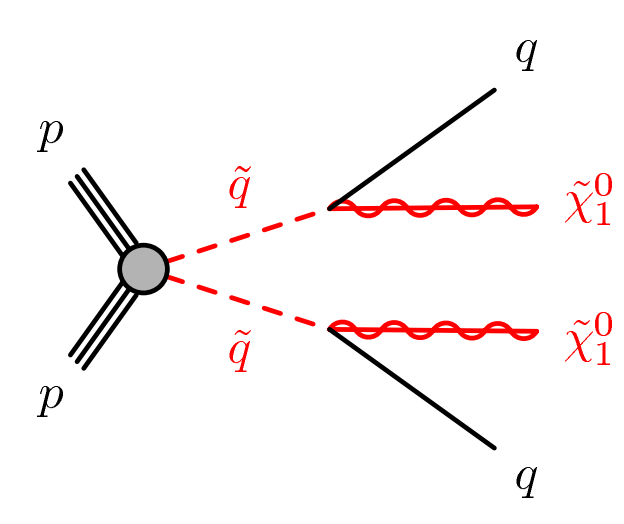
\includegraphics[width=.45\linewidth]{squark_decay}
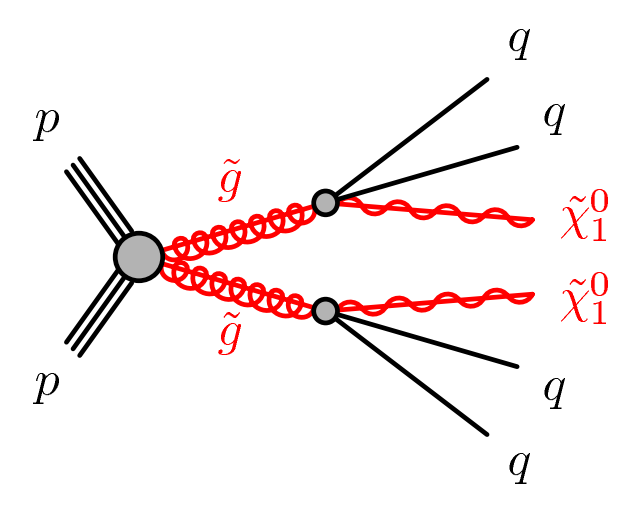
\includegraphics[width=.45\linewidth]{gluino_decay}
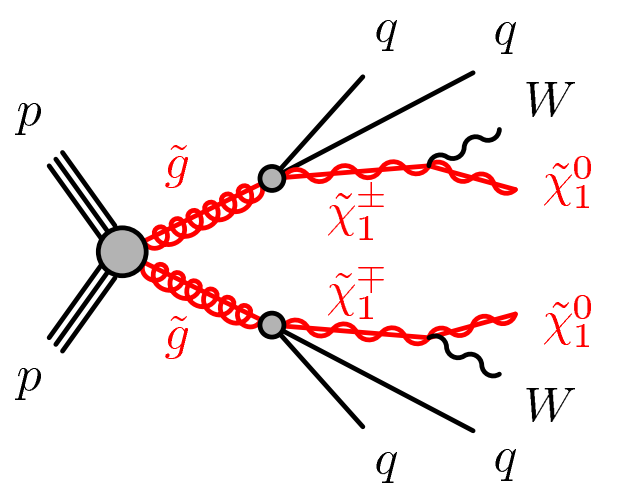
\includegraphics[width=.45\linewidth]{gluino_cascade_w}
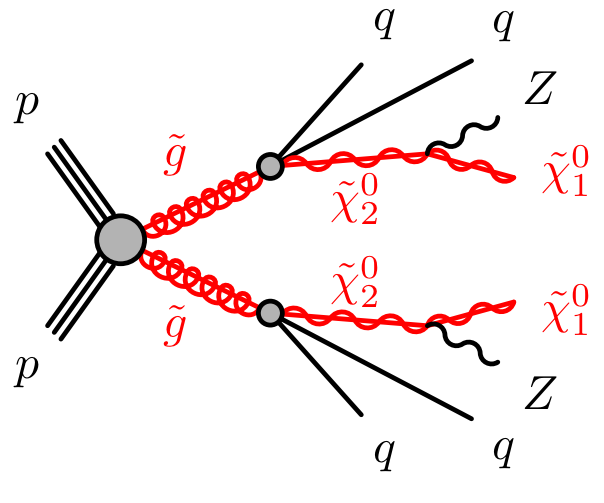
\includegraphics[width=.45\linewidth]{gluino_cascade_z}
\end{figure}
Once we reach the lightest sparticle in the decay, it is absolutely stable.
This leads to the common signature \met for a generic SUSY signal.

For this thesis, we will be presenting an inclusive search for squarks and gluinos with zero leptons in the final state.
This is a very interesting decay channel, due to the high cross-sections of $\supe{g} \supe{g}$ and $\supe{q} \supe{q}$ decays, as can be seen in \Cref{fig:susy_xsec} ~\cite{Borschensky:2014cia}.

\begin{figure}\label{fig:susy_xsec}
\caption{SUSY production cross-sections as a function of sparticle mass at $\sqrt{s} = 13 \TeV$.}
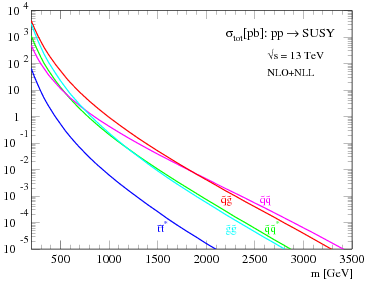
\includegraphics[width=.9\linewidth]{XSectionPlots_13TeV_nlonll_lhc13_col}
\end{figure}
This is a direct consequence of the fact that these are the colored particles of the MSSM.
Since the sparticles interact with the gauge groups of the SM in the same way as their SM partners, the colored sparticles, the squarks and gluinos, are produced and decay as governed by the color group $SU(3)_C$ with the strong coupling $g_S$.
Gluino pair production is particularly copious, due to color factor corresponding to the color octet of $SU(3)_C$.

In the case of squark pair production, the most common decay mode of the squark in the MSSM is a decay directly to the LSP plus a single SM quark ~\cite{susyPrimer}.
This means the basic search strategy for squark pair production is two jets from the final state quarks, plus missing transverse energy from the LSPs.
%There are also cascade decays, the most common of which, and the only one considered in this thesis, is $\supe{q} \rightarrow q \supe{\chi^\pm} \rightarrow q W^\pm \chi^0$.

For gluino pair production, the most common decay is $\supe{g} \rightarrow g \supe{q}$, due to the large $g_S$ coupling.
The squark then decays as listed above.
In this case, we generically search for four jets and missing transverse energy from the LSPs.
%We can also have the squark decay in association with a $W^\pm$ or $Z^0$; in this thesis, we are interested in those cases where this vector boson decays hadronically.

In the context of experimental searches for SUSY, we often consider \textit{simplified models}.
These models make certain assumptions which allow easy comparisons of results by theorists and experimentalists.
In the context of this thesis, the simplified models will make assumptions about the branching ratios described in the preceding paragraphs.
In particular, we will often choose a model where the decay of interest occurs with 100\% branching ratio.
This is entirely for ease of interpretation, but it is important to recognize that these are more a useful comparison tool, especially with for setting limits, than a strict statement about the potential masses of sought-after beyond the Standard Model particle.
%\footnotetext{We will revisit the shortcomings of simplified models in the Conclusion to this thesis.}

\section{How SUSY solves the problems with the SM}

We now return to the issues with the Standard Model as described in \Cref{ch:sm} to see how these issues are solved by supersymmetry.

\subsection{Quadratic divergences to the Higgs mass}

\begin{figure}
\caption{Loop diagrams correct the Higgs mass in the MSSM}\label{fig:susy_loops}
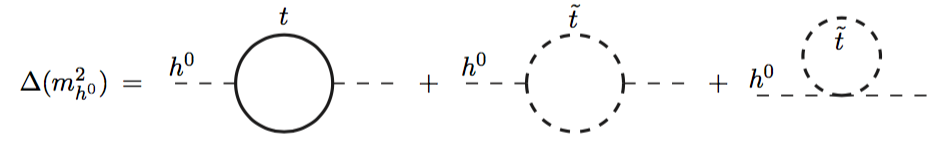
\includegraphics[width=.9\linewidth]{susy_loops}
\end{figure}

The quadratic divergences induced by the loop corrections to the Higgs mass, for example from the top Yukawa coupling, goes as
\begin{equation}
\delta m^2_H \approx \begin{pmatrix} \frac{m_t}{8\pi^2 <\phi>_{VEV}} \end{pmatrix}^2 \Lambda_{Planck}^2.
\end{equation}
The miraculous thing about SUSY is each of these terms \textit{automatically} comes with a term which exactly cancels this contribution~\cite{susyPrimer}.
The fermions and bosons have opposite signs in this loop diagram to all orders in perturbation theory, which completely solves the hierarchy problem.
This is the strongest reason for supersymmetry.

\subsection{Gauge coupling unification}
\begin{figure}
\caption{The running of Standard Model gauge couplings: compare to \Cref{fig:sm_gauge_coupling}.  The MSSM gauge couplings nearly intersect at high energies.}\label{fig:susy_gauge_coupling}
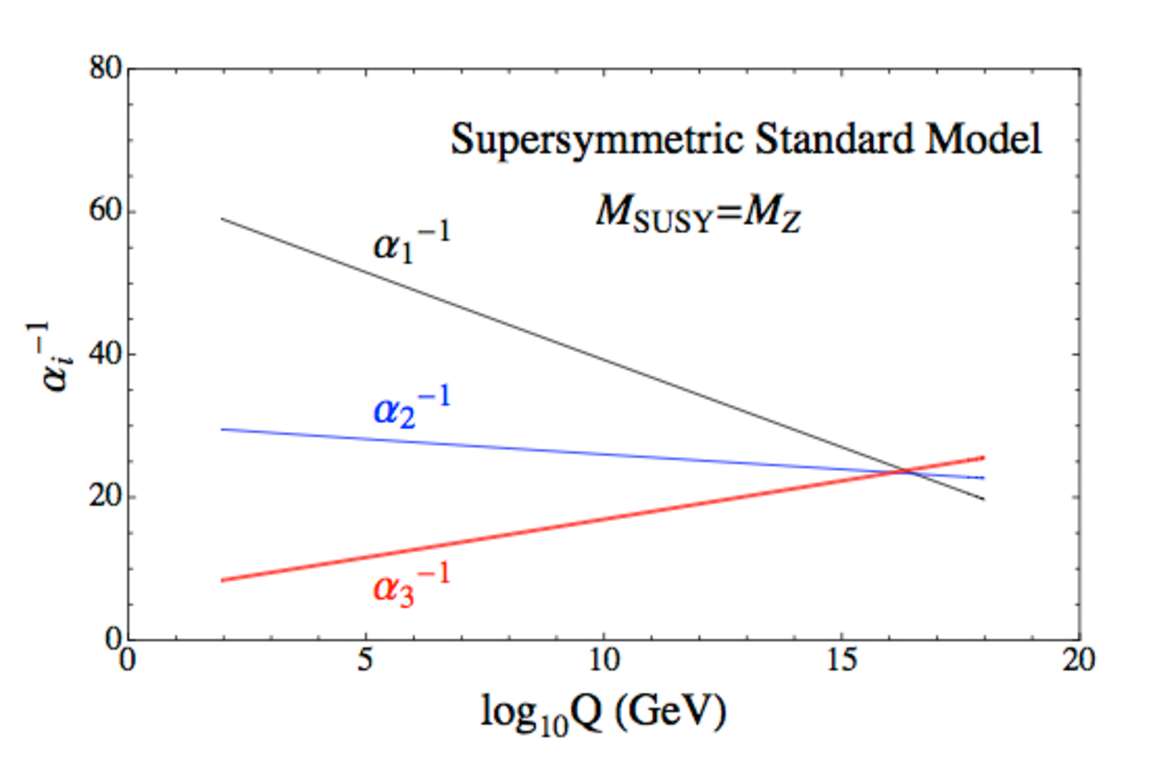
\includegraphics[width=.9\linewidth]{Grand_unification_couplings_susy}
\end{figure}

An additional motivation for supersymmetry is seen by the gauge coupling unification high scales.
In the Standard Model, as we saw the gauge couplings fail to unify at high energies.
In the MSSM and many other forms of supersymmetry, the gauge couplings unify at high energy, as can be seen in \Cref{fig:susy_gauge_coupling}.
This provides additional aesthetic motivation for supersymmetric theories.

\subsection{Dark matter}

As we discussed previously, the lack of any dark matter candidate in the Standard Model naturally leads to beyond the Standard Model theories.
In the Standard Model, there is a natural dark matter candidate in the lightest supersymmetric particle~\cite{susyPrimer}
The LSP would in dark matter experiments be called a  \textit{weakly-interacting massive particle} (WIMP), which is a type of cold dark matter ~\cite{darkMatterPrimer,Klasen:2015uma}.
These WIMPS would only interact through the weak force and gravity, which is exactly as a model like the MSSM predicts for the neutralino.
In \Cref{fig:wimp_exclusions}, we can see the current WIMP exclusions for a given mass.
\begin{figure}
\caption{WIMP exclusions from direct dark matter detection experiments.}\label{fig:wimp_exclusions}
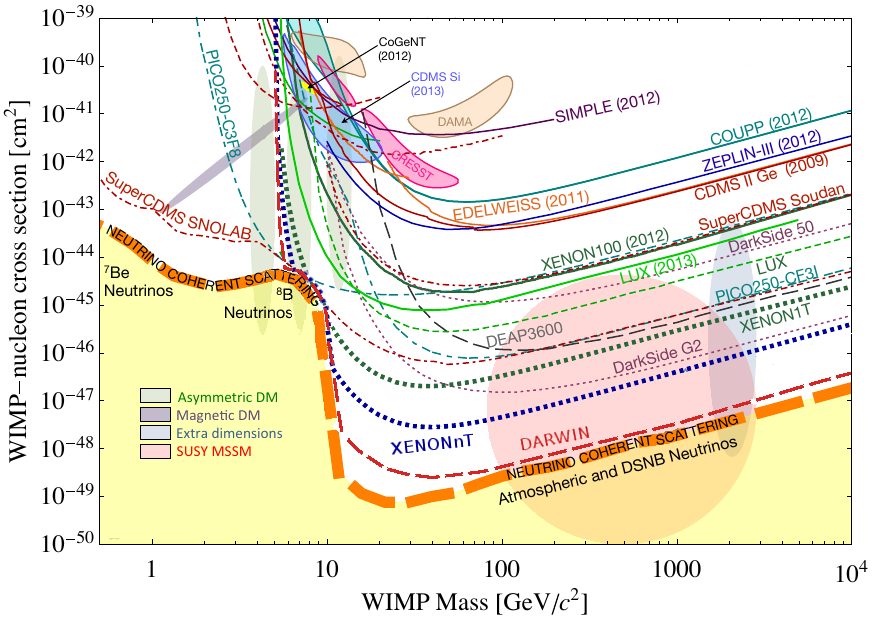
\includegraphics[width=.9\linewidth]{wimp_exclusions}
\end{figure}
The range of allowed masses which have not been excluded for LSPs and WIMPs have significant overlap.
This provides additional motivation outside of the context of theoretical details.

\section{Conclusions}

Supersymmetry is the most well-motivated theory for physics beyond the Standard Model.
It provides a solution to the hierarchy problem, leads to gauge coupling unification, and provides a dark matter candidate consistent with galatic rotation curves.
As noted in this chapter, due to the LSPs in the final state, most SUSY searches require a significant amount of missing transverse energy in combination with jets of high transverse momentum.
However, there is some opportunity to do better than this, especially in final states where one has two weakly-interacting LSPs on opposite sides of some potentially complicated decay tree.
We will see how this is done in \Cref{ch:jigsaw}.
